%=====================================================================
% ANVESH -- IEEE conference paper
% Single self-contained file: paste into Overleaf, no .bib upload needed.
%
% BEFORE SUBMITTING, FILL IN:
%   - institution / department / city / emails in the author block
%   - supervisor acknowledgement (Section ACK)
%   - VERIFY EVERY CITATION in the bibliography. Two are marked
%     "VERIFY" -- we could not confirm exact author/venue/year.
%=====================================================================
\documentclass[conference]{IEEEtran}
\IEEEoverridecommandlockouts

\usepackage{cite}
\usepackage{amsmath,amssymb,amsfonts}
\usepackage{algorithmic}
\usepackage{graphicx}
\usepackage{textcomp}
\usepackage{xcolor}
\usepackage{booktabs}
\usepackage{url}
\usepackage{tikz}
\usetikzlibrary{arrows.meta,positioning}

\def\BibTeX{{\rm B\kern-.05em{\sc i\kern-.025em b}\kern-.08em
    T\kern-.1667em\lower.7ex\hbox{E}\kern-.125emX}}

\begin{document}

\title{Accuracy Is Not Deployability: Measured Failure Modes in an\\
End-to-End Conservation-Aware eDNA Species Identification Pipeline}

\author{
\IEEEauthorblockN{Shriyans Bharuka}
\IEEEauthorblockA{\textit{Dept. of TODO} \\
\textit{TODO Institution}\\
TODO City, India \\
todo@email.com}
\and
\IEEEauthorblockN{Aarya Burande}
\IEEEauthorblockA{\textit{Dept. of TODO} \\
\textit{TODO Institution}\\
TODO City, India \\
todo@email.com}
\and
\IEEEauthorblockN{Darshan Mahale}
\IEEEauthorblockA{\textit{Dept. of TODO} \\
\textit{TODO Institution}\\
TODO City, India \\
todo@email.com}
\linebreakand
\IEEEauthorblockN{Aarav Nambiar}
\IEEEauthorblockA{\textit{Dept. of TODO} \\
\textit{TODO Institution}\\
TODO City, India \\
todo@email.com}
\and
\IEEEauthorblockN{Sunanda Pandit}
\IEEEauthorblockA{\textit{Dept. of TODO} \\
\textit{TODO Institution}\\
TODO City, India \\
todo@email.com}
\and
\IEEEauthorblockN{Leena Madavi}
\IEEEauthorblockA{\textit{Dept. of TODO} \\
\textit{TODO Institution}\\
TODO City, India \\
todo@email.com}
}

\maketitle

%=====================================================================
\begin{abstract}
Environmental DNA (eDNA) metabarcoding promises non-invasive, scalable
biodiversity surveillance, and recent machine learning classifiers report
near-perfect accuracy on marker-gene species identification. We argue that
these headline accuracies systematically overstate what a deployed system
delivers, and we support that argument with measurements from ANVESH, a
complete open eDNA pipeline we built spanning read ingestion, species
classification, conservation-status flagging, biodiversity index
computation, and genetic-similarity visualisation. We benchmark two
independently trained $k$-mer models over 500 marine species drawn from a
curated 12S/16S/COI reference database: a classical 5-mer TF--IDF plus
logistic regression classifier (98.66\% test accuracy) and a compact neural
mean-pooled $k$-mer embedding model (98.85\% test accuracy, 1.14M
parameters). Both are competitive, and both are misleading in isolation. We
then report three failure modes measured on the same held-out data. First,
strand orientation: because read simulators fragment only the forward
strand, a classifier that appears to achieve 98.78\% accuracy collapses to
\textbf{0.38\%} on reverse-complement reads, a failure invisible to standard
evaluation; a training-free dual-orientation inference fix recovers 97.59\%
of those reads at a cost of 1.2 percentage points on forward reads. Second,
a coverage cascade: our model covers 500 of 13{,}351 reference species
(3.7\%), and the conservation-status table intersects only 4 of those 500
(0.8\%), so the conservation feature is effectively inert on arbitrary
input despite being functionally correct. Third, closed-set overconfidence,
which we mitigate with a confidence gate that diverts 89.5\% of
wrong-strand reads away from the reported species list. We additionally
report negative results: an untrained transformer branch, an unintegrated
classical-tool ensemble, and an abandoned quantum-encoding experiment. We
argue that eDNA tooling papers should report orientation robustness and
reference/annotation coverage alongside accuracy, and we release the
pipeline and demonstration dataset to support that.
\end{abstract}

\begin{IEEEkeywords}
environmental DNA, metabarcoding, species identification, marine
biodiversity, $k$-mer classification, deployment, negative results,
conservation informatics
\end{IEEEkeywords}

%=====================================================================
\section{Introduction}

Environmental DNA (eDNA) --- genetic material shed by organisms into water,
soil, or air --- allows biodiversity to be surveyed without observing or
capturing any organism \cite{taberlet2012}. In marine contexts this is
transformative: a water sample can, in principle, reveal the vertebrate
community of a reef, an estuary, or a deep-sea station
\cite{deiner2017,miya2015}. The computational bottleneck is taxonomic
assignment: mapping short marker-gene reads to species. Classical
alignment- and $k$-mer-based tools such as BLAST \cite{blast}, VSEARCH
\cite{vsearch} and Kraken~2 \cite{kraken2} remain the field standard, while
learned models --- from $k$-mer feature classifiers to DNA language models
such as DNABERT \cite{dnabert} and barcode-specific transformers
\cite{barcodebert} --- increasingly report accuracies above 95\% on
curated benchmarks.

We set out to build a deployable system rather than a benchmark entry.
ANVESH ingests raw FASTQ/FASTA reads, classifies them, cross-references each
detected species against IUCN Red List, CITES, and Indian Wildlife
Protection Act records, computes standard biodiversity indices from real
per-sample read counts, and exposes the whole result through a browser
dashboard. Building it end to end surfaced a consistent pattern: every
component was individually correct and individually well-measured, and the
composed system still failed in ways that no component's accuracy metric
predicted.

This paper reports those failures with measurements. Our position is not
that the models are bad --- we report 98.66\% and 98.85\% test accuracy and
we believe those numbers --- but that \emph{accuracy on a held-out split of
simulated forward-strand reads is a weak predictor of behaviour on
deployment input}, and that the eDNA tooling literature does not routinely
report the axes on which that gap appears.

\subsection*{Contributions}
\begin{enumerate}
\item A benchmark of a classical ($k$-mer TF--IDF + logistic regression)
      and a neural (mean-pooled $k$-mer embedding) classifier over 500
      marine species and three marker genes, trained on identical
      simulated data with verified split disjointness
      (Section~\ref{sec:benchmark}).
\item \textbf{A measured strand-orientation failure}: 98.78\%
      $\rightarrow$ 0.38\% accuracy on reverse-complement reads, and a
      training-free dual-orientation inference fix recovering 97.59\% of
      them, with its precision cost quantified
      (Section~\ref{sec:strand}).
\item \textbf{A quantified coverage cascade} showing that a
      conservation-flagging feature can be functionally correct and
      practically inert, with the multiplicative bottleneck measured at
      each stage (Section~\ref{sec:coverage}).
\item An analysis of closed-set overconfidence in eDNA classification and a
      confidence-gated ``unmatched'' pathway that converts silent
      misassignment into an explicit output (Section~\ref{sec:closedset}).
\item \textbf{Negative results}, reported rather than omitted: an untrained
      transformer branch, an unintegrated classical ensemble, and an
      abandoned quantum-encoding experiment (Section~\ref{sec:negative}).
\end{enumerate}

%=====================================================================
\section{Related Work}

\textbf{Classical taxonomic assignment.} BLAST \cite{blast} remains the
reference method for sequence-similarity-based assignment. VSEARCH
\cite{vsearch} provides fast alignment-based clustering and search, and
Kraken~2 \cite{kraken2} performs exact $k$-mer matching against a taxonomic
index. These tools are mature and interpretable but require a curated
reference index at query time and degrade predictably outside it.

\textbf{Learned sequence models.} DNABERT \cite{dnabert} adapted masked
language modelling to genomic $k$-mers. Barcode-specific pretraining
\cite{barcodebert} targets DNA barcoding directly and reports competitive
accuracy against alignment baselines at substantially lower inference cost.
Such models are the natural successor to $k$-mer feature engineering, but
they inherit its closed-set assumption when fine-tuned as classifiers.

\textbf{eDNA pipelines.} Metabarcoding workflows \cite{taberlet2012,
deiner2017} typically chain read quality control, denoising, OTU/ASV
clustering, and reference assignment, with conservation and ecological
interpretation left as manual downstream steps. Marker choice --- 12S for
vertebrate-biased short amplicons \cite{miya2015}, COI as the standard
animal barcode --- materially affects reference availability.

\textbf{Gap.} Reported evaluations focus on assignment accuracy against
held-out reference-derived reads. We are not aware of eDNA classifier
evaluations that report strand-orientation robustness, or that quantify the
downstream annotation coverage that determines whether conservation-aware
features fire at all. Those are the axes this paper measures.

%=====================================================================
\section{System Architecture}
\label{sec:system}

ANVESH is organised as five stages (Fig.~\ref{fig:pipeline}). Reads are
ingested and validated; each read is classified into one of 500 species with
a calibrated confidence; a second, independently trained model embeds the
reads and verifies them against reference centroids in a 192-dimensional
genetic space; biodiversity indices are computed from confident calls; and
each detected species is cross-referenced against conservation records.

\begin{figure}[t]
\centering
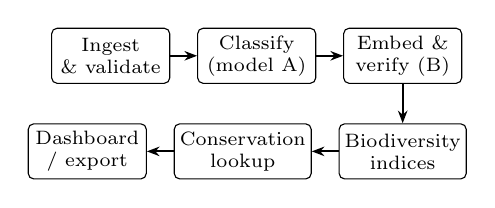
\begin{tikzpicture}[
  node distance=3.4mm,
  box/.style={draw, rounded corners=2pt, align=center, font=\scriptsize,
              minimum height=7mm, minimum width=15mm, inner sep=2pt},
  arr/.style={-{Stealth[length=1.6mm]}, thick}
]
\node[box] (in)  {Ingest\\\& validate};
\node[box, right=of in] (id) {Classify\\(model A)};
\node[box, right=of id] (ve) {Embed \&\\verify (B)};
\node[box, below=5mm of ve] (as) {Biodiversity\\indices};
\node[box, left=of as] (co) {Conservation\\lookup};
\node[box, left=of co] (out) {Dashboard\\/ export};
\draw[arr] (in) -- (id);
\draw[arr] (id) -- (ve);
\draw[arr] (ve) -- (as);
\draw[arr] (as) -- (co);
\draw[arr] (co) -- (out);
\end{tikzpicture}
\caption{ANVESH pipeline. Stage~2 produces the species call; stage~3 is an
independently trained verifier used for similarity, not for the call
itself.}
\label{fig:pipeline}
\end{figure}

\textbf{Ingestion.} FASTA/FASTQ input, optionally gzipped, is parsed as a
stream rather than buffered, and rejected unless at least 90\% of parsed
characters are valid IUPAC nucleotide codes. Both choices were forced by
deployment incidents rather than design foresight
(Section~\ref{sec:resource}).

\textbf{Classification.} Each read receives a species label and the model's
own posterior probability for that label. Reads below a confidence
threshold $\tau=0.5$ are excluded from the species list and from index
computation, and routed to a separate ``unmatched'' output
(Section~\ref{sec:closedset}).

\textbf{Verification.} The embedding model maps reads into 192 dimensions
and computes cosine similarity against precomputed per-species centroids,
yielding both a self-similarity sanity check on the primary call and a
nearest-neighbour list used for visualisation.

\textbf{Ecological assessment.} From confident per-species read counts
$\{n_i\}$ with $p_i = n_i / \sum_j n_j$, we compute richness $S$, the
Shannon index \cite{shannon1948} $H' = -\sum_i p_i \ln p_i$, and Pielou
evenness $J = H'/\ln S$ for $S>1$.

\textbf{Conservation flagging.} Each species is looked up in a locally
cached table; a species is flagged if its IUCN category is CR, EN, or VU, if
its Indian Wildlife Protection Act schedule is I or II, or if it is listed
in CITES Appendix~I. The cache is deliberate: live API dependence would make
field or demonstration use fail on connectivity loss.

%=====================================================================
\section{Dataset and Simulation Methodology}
\label{sec:data}

\subsection{Reference database}
We use a curated marine-vertebrate amplicon reference set
\cite{oceanomics} spanning three marker genes
(Table~\ref{tab:reference}), containing 241{,}990 sequences over 13{,}351
distinct species.

\begin{table}[t]
\caption{Reference database composition}
\label{tab:reference}
\centering
\begin{tabular}{lrr}
\toprule
Marker & Sequences & Distinct species \\
\midrule
12S & 35{,}312 & 8{,}508 \\
16S & 34{,}139 & 7{,}976 \\
COI & 171{,}539 & 11{,}002 \\
\midrule
Union & 241{,}990 & 13{,}351 \\
\bottomrule
\end{tabular}
\end{table}

\subsection{Read simulation}
No real sequencing run was available to us; this is a material limitation
discussed in Section~\ref{sec:threats}. We generate reads by sampling
500 species uniformly at random (seed 42) from the reference union, and for
each species--marker pair extracting 200 fragments of length 150\,bp from
uniformly random start positions, applying an i.i.d.\ substitution error at
rate $\epsilon = 0.005$ per base, and attaching Gaussian-distributed Phred
scores ($\mu = 36$, $\sigma = 3$). This yields 202{,}400 labelled reads
(12S: 58{,}600; 16S: 59{,}800; COI: 84{,}000).

The error model is deliberately simple and is itself a limitation: it
contains no indels, no platform-specific error profile, no chimeras, no PCR
bias, and --- critically for Section~\ref{sec:strand} --- \emph{no
reverse-complement reads}, because fragments are drawn from the forward
strand only. Real amplicon sequencing produces reads from both strands.

\subsection{Splits}
Reads are partitioned 80/10/10 into train/validation/test
(Table~\ref{tab:splits}). We verified zero read-ID overlap and zero exact
sequence overlap between splits. We note that because reads are fragments
of a small number of reference sequences per species, splits share source
sequences even when they share no reads; accuracies should therefore be read
as within-reference generalisation, not cross-population generalisation.

\begin{table}[t]
\caption{Dataset splits (500 species)}
\label{tab:splits}
\centering
\begin{tabular}{lrr}
\toprule
Split & Model A & Model B \\
\midrule
Train      & 161{,}920 & 161{,}889 \\
Validation & 20{,}240  & 20{,}282 \\
Test       & 20{,}240  & 20{,}229 \\
\bottomrule
\end{tabular}
\end{table}

%=====================================================================
\section{Models}
\label{sec:models}

We report four components. Two are trained and deployed; two are not, and we
describe them because their non-completion is part of the result
(Section~\ref{sec:negative}).

\textbf{Model A --- 5-mer TF--IDF + logistic regression.} Reads are encoded
as overlapping 5-mers, weighted by TF--IDF into 1{,}416 features, and
classified by multinomial logistic regression \cite{sklearn}. Inference is
sub-millisecond per read on CPU and requires no accelerator.

\textbf{Model B --- mean-pooled $k$-mer embedding network.} Overlapping
6-mers index a trainable 192-dimensional embedding table; embeddings are
mean-pooled with masking, layer-normalised, and passed through a two-layer
MLP with GELU activation to a 500-way output. The model has 1{,}142{,}516
parameters and was trained for 38 epochs on CPU (best epoch 32, 342\,s total
training time). In deployment we use only the 192-dimensional pooled
representation; its classification head is not used for species calls.

\textbf{Model C --- barcode transformer with recurrent-attention head
(not trained).} We implemented a pretrained barcode transformer
\cite{barcodebert} with a BiLSTM and self-attention classification head.
Only a single-epoch stability run was ever executed; no converged
checkpoint exists. See Section~\ref{sec:negative}.

\textbf{Model D --- classical two-tool ensemble (not integrated).} We
implemented per-marker routing between VSEARCH \cite{vsearch} and Kraken~2
\cite{kraken2} with an agreement-weighted confidence score
($0.6\times$agreement $+\ 0.4\times$identity). It passes its unit checks in
isolation and was never wired into the serving path. See
Section~\ref{sec:negative}.

%=====================================================================
\section{Benchmark Results}
\label{sec:benchmark}

Table~\ref{tab:models} reports held-out performance. Both models exceed
98.6\% accuracy and macro-$F_1$; the neural model is marginally stronger on
macro-$F_1$ (0.9911 vs.\ 0.9895), consistent with better handling of
low-support classes, at roughly $10^3\times$ the parameter count.

\begin{table}[t]
\caption{Held-out performance over 500 species}
\label{tab:models}
\centering
\begin{tabular}{lcc}
\toprule
 & Model A & Model B \\
 & (TF--IDF + LR) & ($k$-mer MLP) \\
\midrule
Parameters        & 1{,}416 feats & 1{,}142{,}516 \\
Validation acc.   & 98.66\% & 98.93\% \\
Test acc.         & 98.66\%$^{\dagger}$ & 98.85\% \\
Test macro-$F_1$  & 0.9895 & 0.9911 \\
Training device   & CPU & CPU \\
Training time     & $<$1\,min & 342\,s \\
\bottomrule
\multicolumn{3}{l}{\footnotesize $^{\dagger}$See Section~\ref{sec:threats}:
this value is identical to the}\\
\multicolumn{3}{l}{\footnotesize validation figure in our stored results and
requires re-verification.}\\
\end{tabular}
\end{table}

The operationally relevant conclusion is not the ranking. It is that a
1{,}416-feature classical model trained in under a minute on a CPU is within
0.2 percentage points of a neural model, on this task and this data. For a
deployment targeting commodity hardware, that difference does not justify
the neural model as the primary classifier --- which is why we deploy Model A
for classification and retain Model B only as an independent verifier.

%=====================================================================
\section{Finding 1: Strand Orientation Collapse}
\label{sec:strand}

\subsection{The failure}
DNA is double-stranded, and amplicon sequencing yields reads from both
strands with no marker in the read indicating which. Our simulator, like
common practice, fragments only the forward strand. A $k$-mer model
therefore never observes reverse-complement $k$-mer profiles during
training. Because reverse-complementation is not an approximate
transformation in $k$-mer space --- it produces an almost entirely disjoint
feature profile --- we hypothesised that the failure would be severe rather
than graceful.

\subsection{Experiment}
We sampled $N=5{,}000$ reads from the held-out test split and evaluated
Model~A under three conditions: \textsc{fwd} (read as given, i.e.\ correct
strand), \textsc{rev} (reverse complement only, simulating a read
sequenced off the opposite strand), and \textsc{dual} (classify both
orientations, keep the higher-confidence call). Ground truth is the
simulator's species label.

\begin{table}[t]
\caption{Strand orientation experiment, $N=5{,}000$ held-out reads}
\label{tab:strand}
\centering
\begin{tabular}{lrrr}
\toprule
Condition & Accuracy & Mean conf. & Conf. $<0.5$ \\
\midrule
\textsc{fwd}  & 98.78\% & 90.94\% & 2.36\% \\
\textsc{rev}  & \textbf{0.38\%} & 26.58\% & 89.50\% \\
\textsc{dual} & 97.58\% & 91.21\% & 1.82\% \\
\bottomrule
\end{tabular}
\end{table}

\subsection{Results}
Table~\ref{tab:strand} shows a near-total collapse: accuracy falls from
98.78\% to 0.38\%, i.e.\ 99.62\% of reverse-strand reads are misassigned.
This is not graceful degradation; it is worse than chance-level performance
would be for a well-calibrated abstaining model, because the model still
produces a confident-looking label.

Two mitigations, measured:

\textbf{(a) Confidence gating.} Mean confidence on wrong-strand reads is
26.58\%, and 89.50\% fall below $\tau=0.5$. The gate therefore intercepts
roughly nine in ten wrong-strand reads before they reach the reported
species list --- valuable, but it still leaks the remaining tenth as
confident errors.

\textbf{(b) Dual-orientation inference.} Classifying both orientations and
keeping the higher-confidence call recovers 97.59\% of the reads that
reverse-strand input would have lost, requires no retraining, and doubles
inference cost (negligible here: Model~A is sub-millisecond per read).

\subsection{The cost, reported honestly}
Dual-orientation inference is not free. On known-forward reads accuracy
falls from 98.78\% to 97.58\%, a loss of 1.20 percentage points, because
the reverse complement occasionally attracts spuriously higher confidence
than the correct forward call. The trade is 1.2 points of precision on
correctly-oriented input in exchange for approximately 97 points of recall
on incorrectly-oriented input. For any pipeline whose input orientation is
unknown --- which is every real eDNA pipeline --- this is strongly
favourable, but it should be stated rather than absorbed silently.

\subsection{Implication}
The deeper point is about evaluation, not about the fix. A held-out split
drawn from a forward-only simulator cannot expose this failure: the test set
inherits the training set's orientation bias, so the reported 98.66\%
measures a condition the deployed system never encounters in pure form. We
suggest that eDNA classifier evaluations report reverse-complement accuracy
as a standard secondary metric, and that simulators either emit both
strands or document that they do not.

%=====================================================================
\section{Finding 2: The Coverage Cascade}
\label{sec:coverage}

Conservation-aware identification is a common motivation for eDNA tooling.
We implemented it, verified it end to end, and found it almost never fires.
The cause is a multiplicative coverage cascade
(Table~\ref{tab:coverage}).

\begin{table}[t]
\caption{Coverage cascade from reference to actionable flag}
\label{tab:coverage}
\centering
\begin{tabular}{lrr}
\toprule
Stage & Species & \% of previous \\
\midrule
Reference database          & 13{,}351 & --- \\
Model output vocabulary     & 500      & 3.7\% \\
$\cap$ conservation records & 4        & 0.8\% \\
\bottomrule
\end{tabular}
\end{table}

Two independent bottlenecks compose. The classifier is closed-set over the
500 species sampled for training, i.e.\ 3.7\% of the reference database. The
conservation table, hand-curated from IUCN, CITES and Indian Wildlife
Protection Act sources, contained 21 species. The intersection --- species
the model can emit \emph{and} the table can annotate --- was originally a
single species, and 4 after we deliberately extended the table toward the
model's vocabulary.

The consequence is a feature that is individually correct and jointly
inert. We verified the flagging path end to end: a genuine reference-derived
read of \textit{Carcharhinus longimanus} (IUCN Critically Endangered)
classifies at 99.1\% confidence and is correctly flagged. Yet the
probability that an arbitrary input triggers any flag is governed by the
0.8\% intersection, not by the correctness of the lookup. Well-known
conservation targets present in the curated table --- whale shark, several
sea turtles, dugong --- lie outside the model's vocabulary entirely and can
therefore \emph{never} be reported, regardless of input.

We stress the asymmetry in curation cost. Extending the annotation table is
cheap: it is a data file, and we added three verified species in minutes
without retraining or redeployment. Extending the model's vocabulary
requires retraining. Where the two sets are curated independently --- which
is the natural division of labour between domain and ML contributors --- the
intersection is not optimised by either, and can approach zero without any
individual component being wrong. We recommend that conservation-aware
pipelines report intersection coverage explicitly, and that annotation
curation be driven by the model vocabulary rather than by taxonomic
prominence.

%=====================================================================
\section{Finding 3: Closed-Set Overconfidence}
\label{sec:closedset}

A softmax classifier over 500 species must assign one of them to every
input. It has no abstention mechanism, so an unrepresented organism --- the
common case in a database covering 3.7\% of reference species, and the
scientifically interesting case in eDNA generally --- receives a confident
label rather than a null result. Section~\ref{sec:strand} demonstrates the
extreme form: 99.62\% of wrong-strand reads receive a wrong species label.

We adopt an explicit gate at $\tau=0.5$. Reads below threshold are excluded
from the species list and from all biodiversity index computation, and are
emitted as a distinct ``unmatched'' output, grouped by nearest rejected
species and accompanied by the embedding-space nearest neighbours from
Model~B. Two properties matter. First, ecological indices computed over
gated reads are not contaminated by low-confidence assignments, which would
otherwise inflate richness --- the metric most sensitive to spurious
singletons. Second, the unmatched output is presented as a positive
result: sequences that plausibly correspond to unrepresented, under-sequenced,
or novel taxa are the scientifically valuable residue of a survey, and
silently mislabelling them as known species destroys exactly the signal a
biodiversity survey exists to find.

We do not claim $\tau=0.5$ is optimal; it was not tuned against a
labelled open-set benchmark, because we had none. Establishing calibrated
open-set thresholds for eDNA classification is future work.

%=====================================================================
\section{Finding 4: Resource-Driven Constraints}
\label{sec:resource}

Two implementation constraints emerged from deploying on free-tier
commodity infrastructure, and both changed the system design.

\textbf{Memory.} An early implementation buffered the uploaded file before
parsing. A 135\,MB uncompressed reference upload exhausted the 512\,MB
container and terminated the process before classification began. Parsing
was rewritten as a line-oriented stream with early termination once the
read cap is reached, including for gzipped input, where decompression also
halts early. Peak memory is now independent of input size.

\textbf{Compute.} Both deployed models run on CPU. Model~B is trained and
served with a CPU-only build of the deep learning framework, roughly an
order of magnitude smaller than the accelerator-enabled distribution and
the only variant that fit the deployment's image budget. This constrained
model selection --- and, combined with the benchmark of
Section~\ref{sec:benchmark}, is the substantive reason a 1{,}416-feature
classical model serves production traffic while a neural model is relegated
to verification. We note that hardware constraints of this kind are typical
of the field deployments eDNA tooling targets, and that reporting accuracy
without inference cost obscures which model is actually deployable.

%=====================================================================
\section{Negative Results}
\label{sec:negative}

We report three components that did not reach deployment. We include them
because their omission would misrepresent both the effort distribution of
the project and the difficulty of the tasks.

\textbf{Transformer branch (Model C).} We integrated a pretrained barcode
transformer \cite{barcodebert} with a BiLSTM and self-attention head, and
verified that the architecture executes end to end. It was never trained to
convergence: only a single-epoch, 100-batch stability run was performed, and
no usable checkpoint exists. The blocker was compute and calendar time, not
a defect in the approach --- published results for barcode-specific
transformers are strong \cite{barcodebert}, and we expect this branch to
outperform Model~A if trained. We report it as unfinished rather than as a
result, and note that the classical baseline's competitiveness
(Section~\ref{sec:benchmark}) reduced the marginal urgency of finishing it.

\textbf{Classical ensemble (Model D).} The VSEARCH/Kraken~2 router and its
agreement-weighted confidence score were implemented and unit-checked, but
never integrated into the serving path, because doing so required
provisioning and invoking two external tool binaries per request within the
deployment's resource envelope. This is a systems-integration failure, not
an algorithmic one, and it is precisely the class of failure that separates
a working component from a deployed one.

\textbf{Quantum encoding experiment.} We explored quantum autoencoders for
novelty detection over sequence representations, motivated by the open-set
problem of Section~\ref{sec:closedset}. At the qubit counts available to us
the approach did not produce usable separation, with circuit noise dominating
the signal at the encoding widths required for realistic sequence
representations. We report this as a negative result: we do not currently
see a route by which quantum encoding improves eDNA novelty detection at
presently available scales, and we would discourage others from treating it
as low-hanging fruit.

%=====================================================================
\section{Limitations and Threats to Validity}
\label{sec:threats}

\textbf{No real sequencing data.} This is the dominant limitation. Every
number in this paper derives from simulated reads. Our error model omits
indels, platform-specific error profiles, PCR and primer bias, chimeras,
and contamination. Real Illumina or Nanopore output will differ, and our
absolute accuracies should be treated as upper bounds on a favourable
distribution. We expect the \emph{direction} of Finding~1 to survive contact
with real data --- reverse-complement reads genuinely occur, and the model
genuinely never saw them --- but its magnitude on real reads is unmeasured.

\textbf{Split independence.} Splits share source reference sequences even
though they share no reads or exact sequences. Reported accuracy therefore
measures within-reference generalisation and likely overstates performance
on populations divergent from the reference.

\textbf{A metric inconsistency.} Our stored evaluation record for Model~A
lists identical validation and test accuracy (0.9865612648221344) while
listing distinct macro-$F_1$ values. We believe the accuracy field was
duplicated rather than independently computed. We report the value as
published in our artefacts and flag it as requiring re-verification rather
than silently correcting or omitting it; Model~A's accuracy should be
treated as approximate at the second decimal place. The strand experiment of
Section~\ref{sec:strand} was run fresh against the stored model and is
unaffected.

\textbf{Conservation data provenance.} Of 21 conservation records, 18 were
manually verified against primary sources; 3 were added later to enable
end-to-end demonstration and are marked in our artefacts as requiring
verification before citation. No conservation claim in this paper depends
on the unverified three.

\textbf{Single reference database.} All results derive from one curated
marine-vertebrate amplicon set. Generalisation to other reference
databases, taxa, or marker genes is untested.

%=====================================================================
\section{Future Work}

The immediate priority is validation on real sequencing output, without
which Finding~1's magnitude and the benchmark's absolute values remain
provisional. Second, reverse-complement augmentation at training time should
be compared directly against our inference-time fix: augmentation should
recover the 1.2-point precision cost, at the price of retraining.
Third, open-set methods --- calibrated abstention, or distance-based
novelty detection over Model~B's embedding space --- would replace the
hand-set threshold of Section~\ref{sec:closedset} with a principled
rejection criterion. Fourth, the coverage cascade motivates
vocabulary-driven annotation curation, and a larger training vocabulary
approaching the reference database's 13{,}351 species. Finally, completing
the transformer branch would test whether barcode-specific pretraining's
reported advantages hold under the deployment constraints of
Section~\ref{sec:resource}.

%=====================================================================
\section{Conclusion}

We built a complete conservation-aware eDNA identification pipeline and
measured where it fails. Two $k$-mer classifiers reach 98.66\% and 98.85\%
accuracy over 500 marine species, and neither number predicts deployment
behaviour. Reverse-complement reads --- which every real amplicon run
produces and which forward-only simulators never generate --- reduce
accuracy to 0.38\%, recoverable to 97.58\% by dual-orientation inference at
a measured 1.2-point precision cost. A correctly implemented conservation
flagging feature fires on 0.8\% of the model's vocabulary because two
independently curated sets barely intersect. A closed-set classifier assigns
confident labels to organisms it has never seen, mitigated but not solved by
confidence gating. We additionally report an untrained transformer branch,
an unintegrated classical ensemble, and a failed quantum encoding
experiment.

The pattern across all four findings is the same: each component was
individually correct, and the composed system still failed. We suggest that
eDNA tooling evaluations report orientation robustness, intersection
coverage, and open-set behaviour alongside accuracy, and that negative
results of the kind reported here be published rather than discarded, since
they describe precisely the gap between a benchmark result and a deployable
system.

%=====================================================================
\section*{Acknowledgment}

The authors thank TODO~SUPERVISOR~NAME for guidance and for encouraging the
publication of the negative results reported in Section~\ref{sec:negative}.
TODO: add any institutional or funding acknowledgements.

%=====================================================================
\begin{thebibliography}{00}

\bibitem{taberlet2012} P. Taberlet, E. Coissac, M. Hajibabaei, and L. H.
Rieseberg, ``Environmental DNA,'' \emph{Molecular Ecology}, vol. 21, no. 8,
pp. 1789--1793, 2012.

\bibitem{deiner2017} K. Deiner \emph{et al.}, ``Environmental DNA
metabarcoding: transforming how we survey animal and plant communities,''
\emph{Molecular Ecology}, vol. 26, no. 21, pp. 5872--5895, 2017.

\bibitem{miya2015} M. Miya \emph{et al.}, ``MiFish, a set of universal PCR
primers for metabarcoding environmental DNA from fishes,'' \emph{Royal
Society Open Science}, vol. 2, no. 7, 150088, 2015.

\bibitem{blast} S. F. Altschul, W. Gish, W. Miller, E. W. Myers, and D. J.
Lipman, ``Basic local alignment search tool,'' \emph{Journal of Molecular
Biology}, vol. 215, no. 3, pp. 403--410, 1990.

\bibitem{vsearch} T. Rognes, T. Flouri, B. Nichols, C. Quince, and F.
Mah\'e, ``VSEARCH: a versatile open source tool for metagenomics,''
\emph{PeerJ}, vol. 4, e2584, 2016.

\bibitem{kraken2} D. E. Wood, J. Lu, and B. Langmead, ``Improved
metagenomic analysis with Kraken 2,'' \emph{Genome Biology}, vol. 20, no. 1,
257, 2019.

\bibitem{dnabert} Y. Ji, Z. Zhou, H. Liu, and R. V. Davuluri, ``DNABERT:
pre-trained bidirectional encoder representations from transformers model
for DNA-language in genome,'' \emph{Bioinformatics}, vol. 37, no. 15, pp.
2112--2120, 2021.

\bibitem{barcodebert} % VERIFY: confirm authors, venue and year before submission.
Authors TODO, ``BarcodeBERT: transformers for biodiversity analysis,''
TODO venue, TODO year. [Online]. Available:
\url{https://huggingface.co/bioscan-ml/BarcodeBERT}

\bibitem{oceanomics} % VERIFY: confirm the correct citation for this reference set.
OceanOmics, ``OceanOmics amplicon reference database,'' TODO year. [Online].
Available: TODO URL

\bibitem{shannon1948} C. E. Shannon, ``A mathematical theory of
communication,'' \emph{Bell System Technical Journal}, vol. 27, no. 3, pp.
379--423, 1948.

\bibitem{sklearn} F. Pedregosa \emph{et al.}, ``Scikit-learn: machine
learning in Python,'' \emph{Journal of Machine Learning Research}, vol. 12,
pp. 2825--2830, 2011.

\bibitem{umap} L. McInnes, J. Healy, and J. Melville, ``UMAP: uniform
manifold approximation and projection for dimension reduction,''
\emph{arXiv:1802.03426}, 2018.

\bibitem{iucn} IUCN, ``The IUCN Red List of Threatened Species.'' [Online].
Available: \url{https://www.iucnredlist.org}

\bibitem{gbif} GBIF, ``Global Biodiversity Information Facility occurrence
data.'' [Online]. Available: \url{https://www.gbif.org}

\end{thebibliography}

\end{document}
